\chapter{提案手法}\label{chap:method}

\section{提案手法の概要}

1章の背景で述べたような分岐路において,ルートを選択する場合に
入力する情報としてカメラ画像のみでは「右と左のどちらに曲がる」という判断をするための情報が不足していると考えられる.
そこで,カメラ画像をもとにEnd-to-End学習で経路追従行動を行う
従来研究\cite{okada}で用いたシステムへカメラ画像以外にルートの選択に必要な情報として,「直進」「左折」「右折」の目標方向情報をコマンドを追加した,
提案手法の概要を以下に示す
学習フェーズ
テストフェーズ
本研究で対象とするロボットの構造,搭載するセンサを\ref{fig::turtlebot3_gazo}に示す.

\begin{figure}[H]
    \centering
    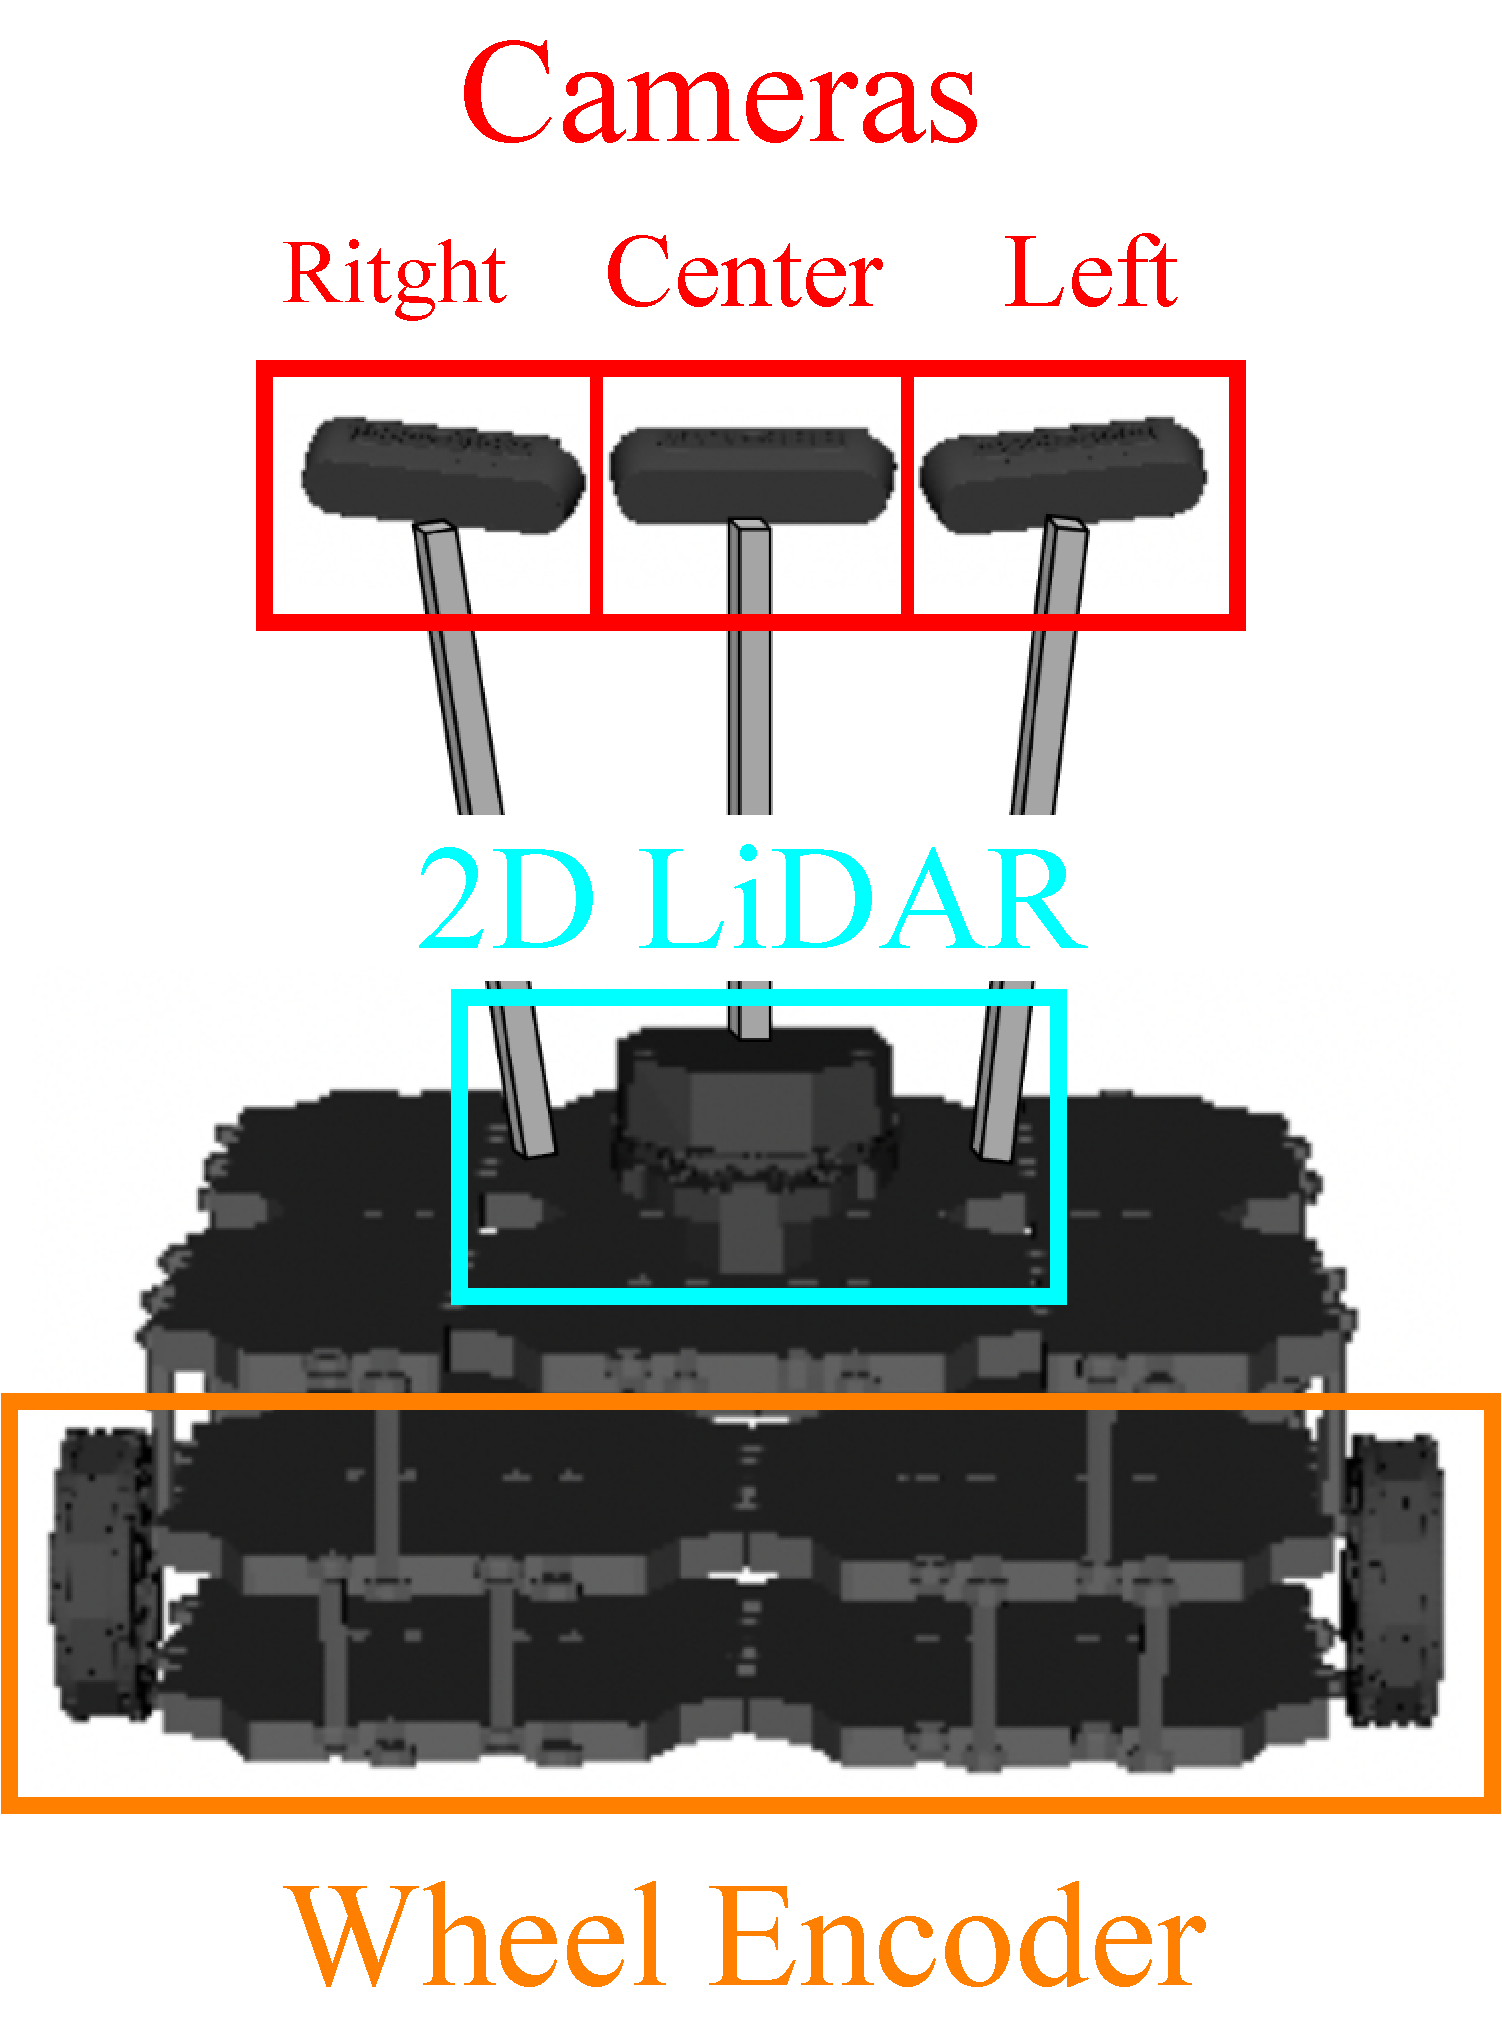
\includegraphics[width = 4cm]{./figs/turtlebot3_kame.pdf}
    \caption{turtlebot3 waffle}
    \label{fig::turtlebot3_gazo}
\end{figure}


% \begin{table}[ht]
%     \centering
%     \caption{Robot}
%       \begin{tabular}{c|cll}
%       \hline
%       tpye    & Differential-drive wheele                                                           \\ \hline
%       sensors & \begin{tabular}[c]{@{}l@{}}2D-LiDAR\\ Wheel Encoder\\ Monocular Camera\end{tabular} \\ \hline
%       \end{tabular}

    
%     \label{tb:hikaku}
   
%     \end{table}


\begin{figure}[H]
    \begin{tabular}{c}
      \begin{minipage}[t]{0.5\hsize}
        \centering
        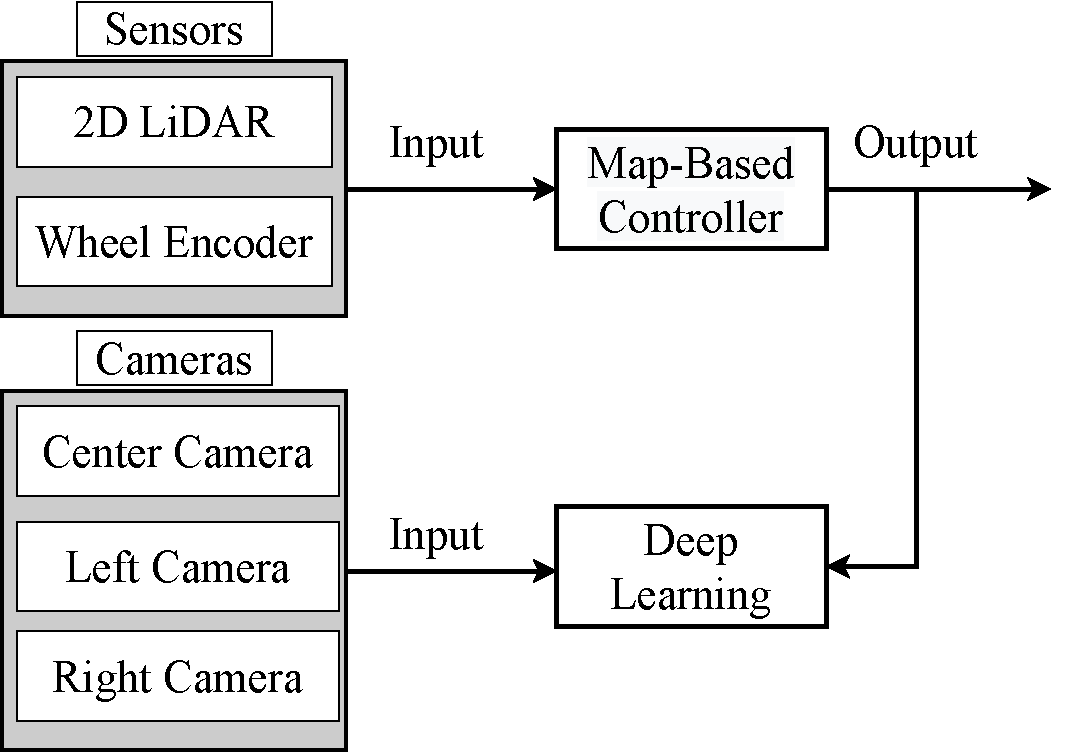
\includegraphics[keepaspectratio, scale=0.4]{./figs/system_abs.pdf}
        \subcaption{Learning system}
        \label{exp29}
      \end{minipage}\\
      \begin{minipage}[t]{0.5\hsize}
        \centering
        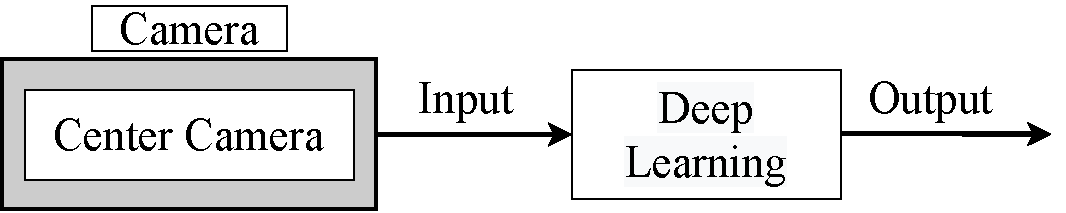
\includegraphics[keepaspectratio, scale=0.4]{./figs/system_test_abs.pdf}
        \subcaption{Test system}
        \label{exp28}
      \end{minipage} \\
      \vspace{2.0zh}
    \end{tabular}
     \caption{Experiment 2 route}
     \label{fig::exp20}
  \end{figure}

\newpage
\section{システム}
本研究室のチームが行ってきたシステム\cite{okada}へ目標方向に対応したコマンドの生成機能とネットワーク構造の変更をすることでシステムを構築した.
「道なり」「直進」「左折」「右折」の目標方向を要素数3,次元数1のint型の配列(One-Hot ベクトル)で表現し,方向と配列の対応をTable \ref{tb:comman}に示す.

本節では学習器の訓練を行う\ref{lerning}「学習フェーズ」,学習結果を用いて走行を行う\ref{test}「テストフェーズ」,
\ref{net}構築したネットワークの構造と\ref{seigyo}学習フェーズで用いる地図べースの制御器の4つに分けて述べる.
\vspace{2.0zh}
\begin{table}[h]
    \centering
    \caption{Command}
    \begin{tabular}{cccll}
    \cline{1-4}
    \multicolumn{1}{|c|}{Target Direction} & \multicolumn{1}{c|}{go straihgt}          & \multicolumn{1}{c|}{go left}          & \multicolumn{1}{c|}{go right}          &  \\ \cline{1-4}
    \multicolumn{1}{|c|}{data}  & \multicolumn{1}{c|}{{[} 100, 0, 0 {]}} & \multicolumn{1}{c|}{{[} 0, 100, 0 {]}} & \multicolumn{1}{l|}{{[} 0, 0, 100 {]}} &  \\ \cline{1-4}
                               &                                  &                                  &                                  &  \\
                               &                                  &                                  &                                  &  \\
    \multicolumn{1}{l}{}       &                                  &                                  &                                  & 
    \end{tabular}
    \vspace{-3.0zh}
    \label{tb:comman}
    \end{table}
  
    \begin{table}[h]
      \centering
      \caption{Command}
      \begin{tabular}{ccccll}
      \cline{1-5}
      \multicolumn{1}{|c|}{Target Direction} & \multicolumn{1}{c|}{con}&\multicolumn{1}{c|}{go straihgt}          & \multicolumn{1}{c|}{go left}          & \multicolumn{1}{c|}{go right}          &  \\ \cline{1-5}
      \multicolumn{1}{|c|}{data}  &\multicolumn{1}{c|}{{[}100, 0, 0, 0{]}}& \multicolumn{1}{c|}{{[}100, 0, 0, 0{]}} & \multicolumn{1}{c|}{{[}0,100,0, 0{]}} & \multicolumn{1}{l|}{{[}0, 0, 0, 100{]}} &  \\ \cline{1-5}
                                 &                                  &                                  &                                  &  \\
                                 &                                  &                                  &                                  &  \\
      \multicolumn{1}{l}{}       &                                  &                                  &                                  & 
      \end{tabular}
      \vspace{-3.0zh}
      \label{tb:command_4}
      \end{table}
  
\newpage
\section{地図ベースの制御器}
    \label{seigyo}
    学習フェーズで使用する地図ベースの制御器について,概要をFig. \ref{fig::navigation}に示す.
    センサからの観測情報を用いて局所的な障害物認識を行うlocal\_costmap,local\_costmapの結果を利用して局所的な経路計画を行うlocal\_planner.
    後述するmap\_serverから配信される,地図に対して全体のコスト計算を行うglobal\_costmap.
    その結果を利用して大域的な経路計画を行うglobal\_plannner.
    これらをレイヤーとして統合して行動計画とモータ指令を行う「move\_base」,Particle\_Filterによって自己位置推定を行う「amcl」,2つへ保持する地図の配信を行う
    「map\_server」などのパッケージを統合した自律移動用のメタパッケージである
    ROS Navigation\_stack\cite{navigation:online}へ目標地点(waypoint)とコマンドの生成機能をもつ「waypoint\_nav」を組み込んで使用している.
    \vspace{2.0zh}
    \begin{figure}[h]
        \centering
        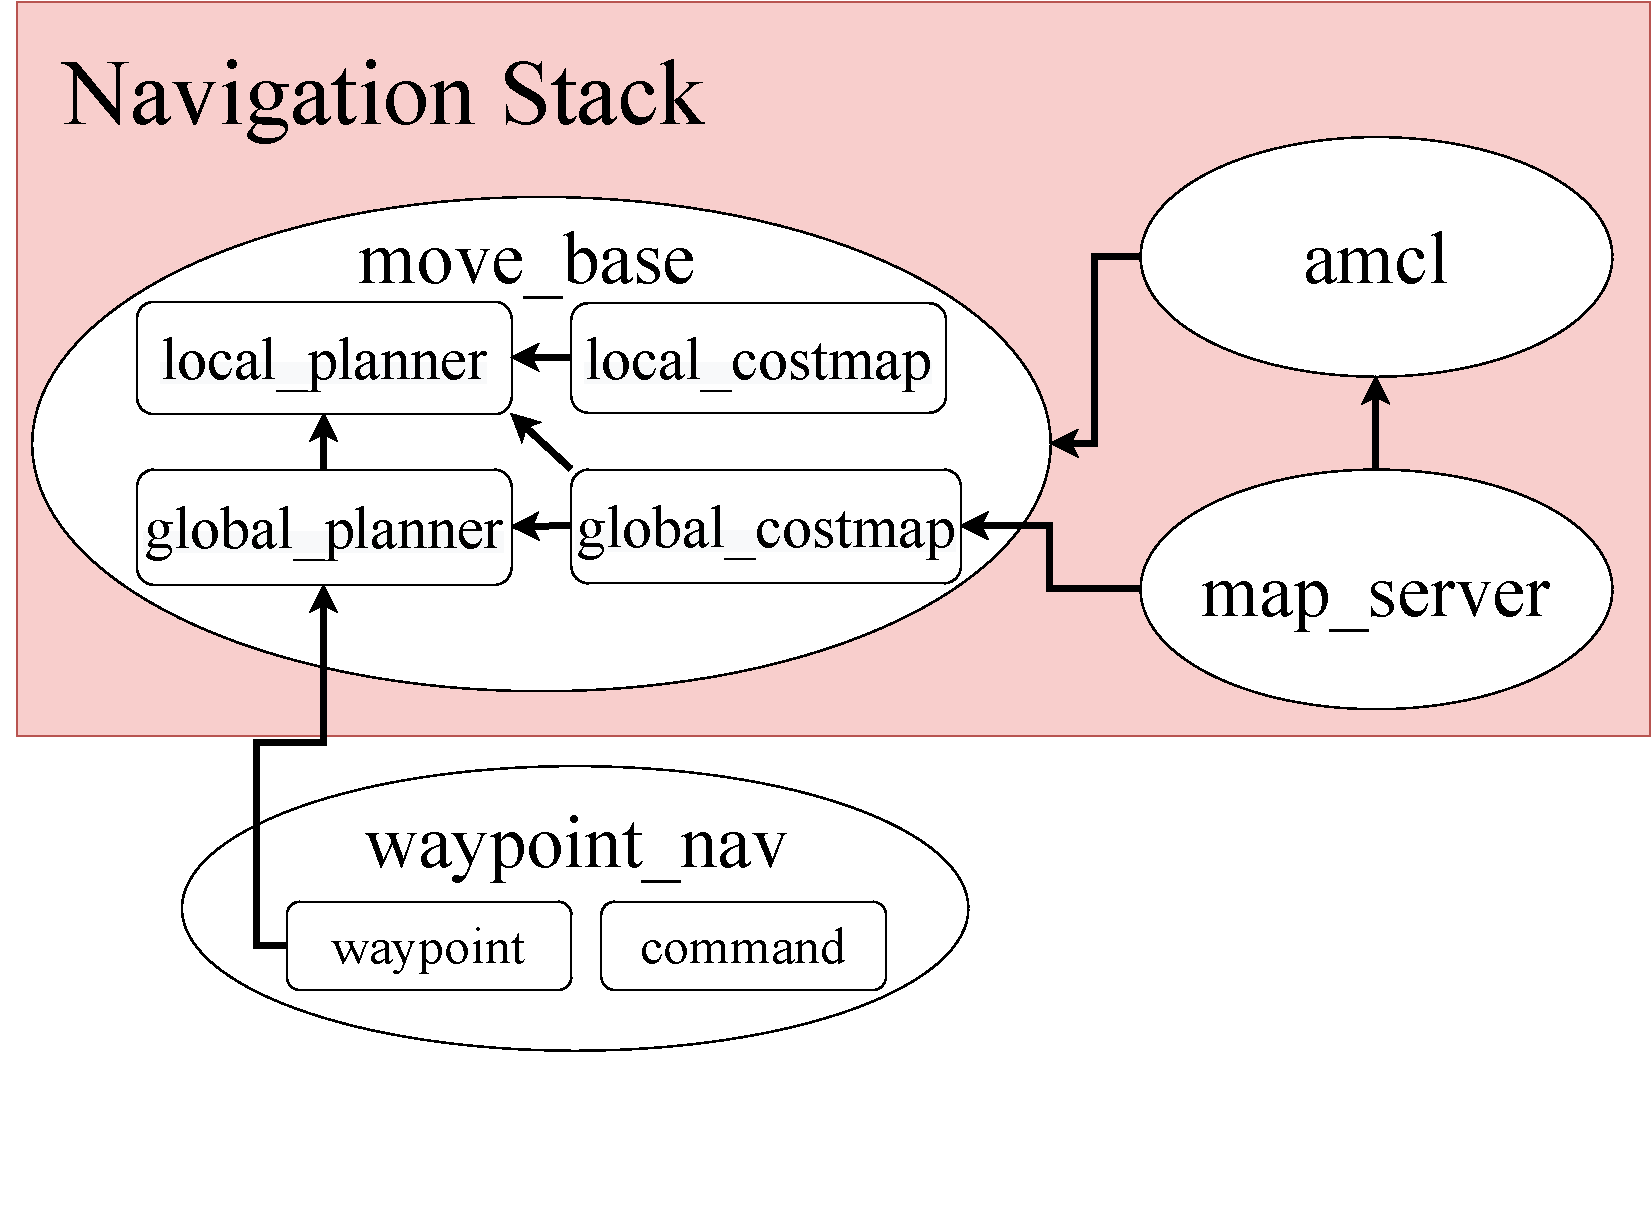
\includegraphics[width = 12cm]{./figs/navigation.pdf}
        \caption{Map-based controller}
        \label{fig::navigation}
    \end{figure}


\newpage

\subsection{学習フェーズ}
\label{lerning}
学習器の訓練を行う学習フェーズで用いるシステムをFig. \ref{fig::learningsystem}示す.
学習は下記の一連の流れを1stepとして,設定したstep数行う.
\begin{enumerate}
    \item LiDARとオドメトリを入力とする地図ベースの制御器の出力を用いて自律走行を行う
    \item 地図ベースの制御器の出力からヨー方向の角速度とコマンド,機体に取り付けたカメラからRGB画像を取得し,訓練データへ加える
    \item 訓練データを 入力:カメラ画像,コマンド 目標出力:角速度 として学習器へ渡す
    \item 学習器の出力を記録.
  \end{enumerate}
画像の取得には従来研究\cite{okada}にならって,機体の中央, 中央に対して左,右に傾けて取り付けた3つのカメラを用いる.
また分岐路以外では,1つのコマンド(例として「直進」)を出力し続けた場合にデータセットへ偏りが生じる可能性が考えられるため,
ランダムなコマンドの出力を用いる.
コマンドの生成方法は\ref{seigyo}で述べるwaypointを用いて,目標方向に対応したコマンドを生成する.

\begin{figure}[H]
    \centering
    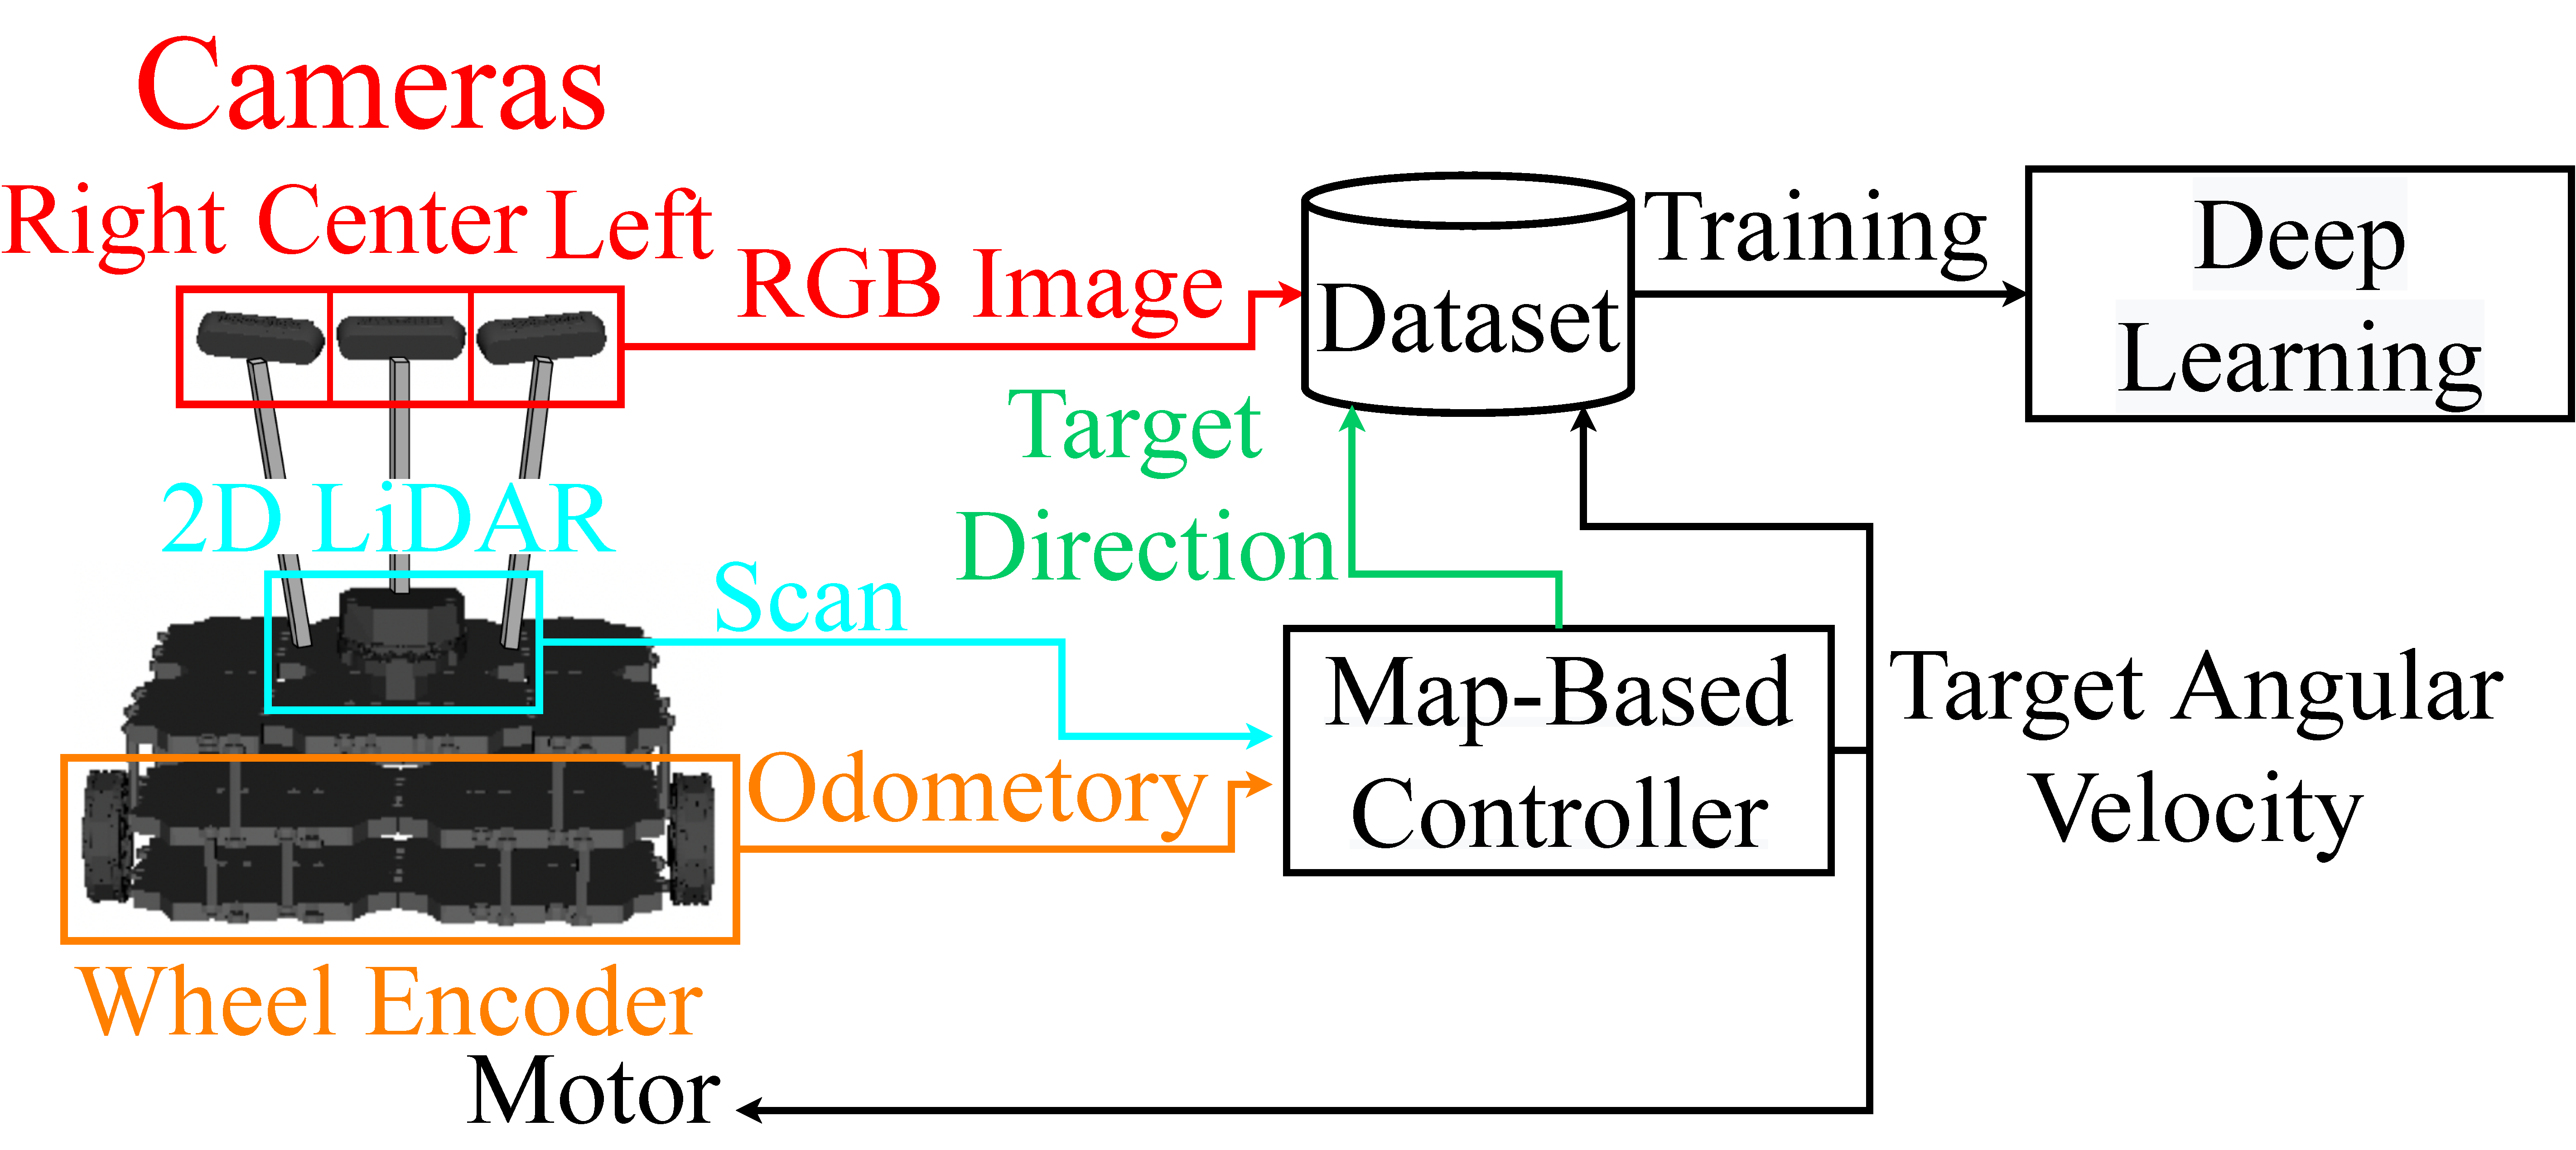
\includegraphics[width = 12cm]{./figs/system_learning.pdf}
    \caption{Learning system }
    \label{fig::learningsystem}
\end{figure}


\newpage
\subsection{テストフェーズ}
\label{test}
設定したstep数に達した場合に,Fig. \ref{fig::testsystem}に示すように
地図ベースの制御器の出力による動作から,中央のカメラ画像とコマンドを入力とした
学習器の出力による動作へ切り替えて走行を行う.
テスト時のコマンドの生成(方向の指示)はJoy\_stickコントローラのボタンを用いて行う.
テストフェーズにおける手順を下記に示す.
\begin{enumerate}
    \item 機体に取り付けた中央のカメラからRGB画像,Joy\_stickコントローラよりコマンドのデータを取得
    \item 取得したデータ(カメラ画像,コマンド)を学習器へ入力
    \item 学習器の出力である角速度をモータへ与える
  \end{enumerate}


\begin{figure}[h]
    \centering
    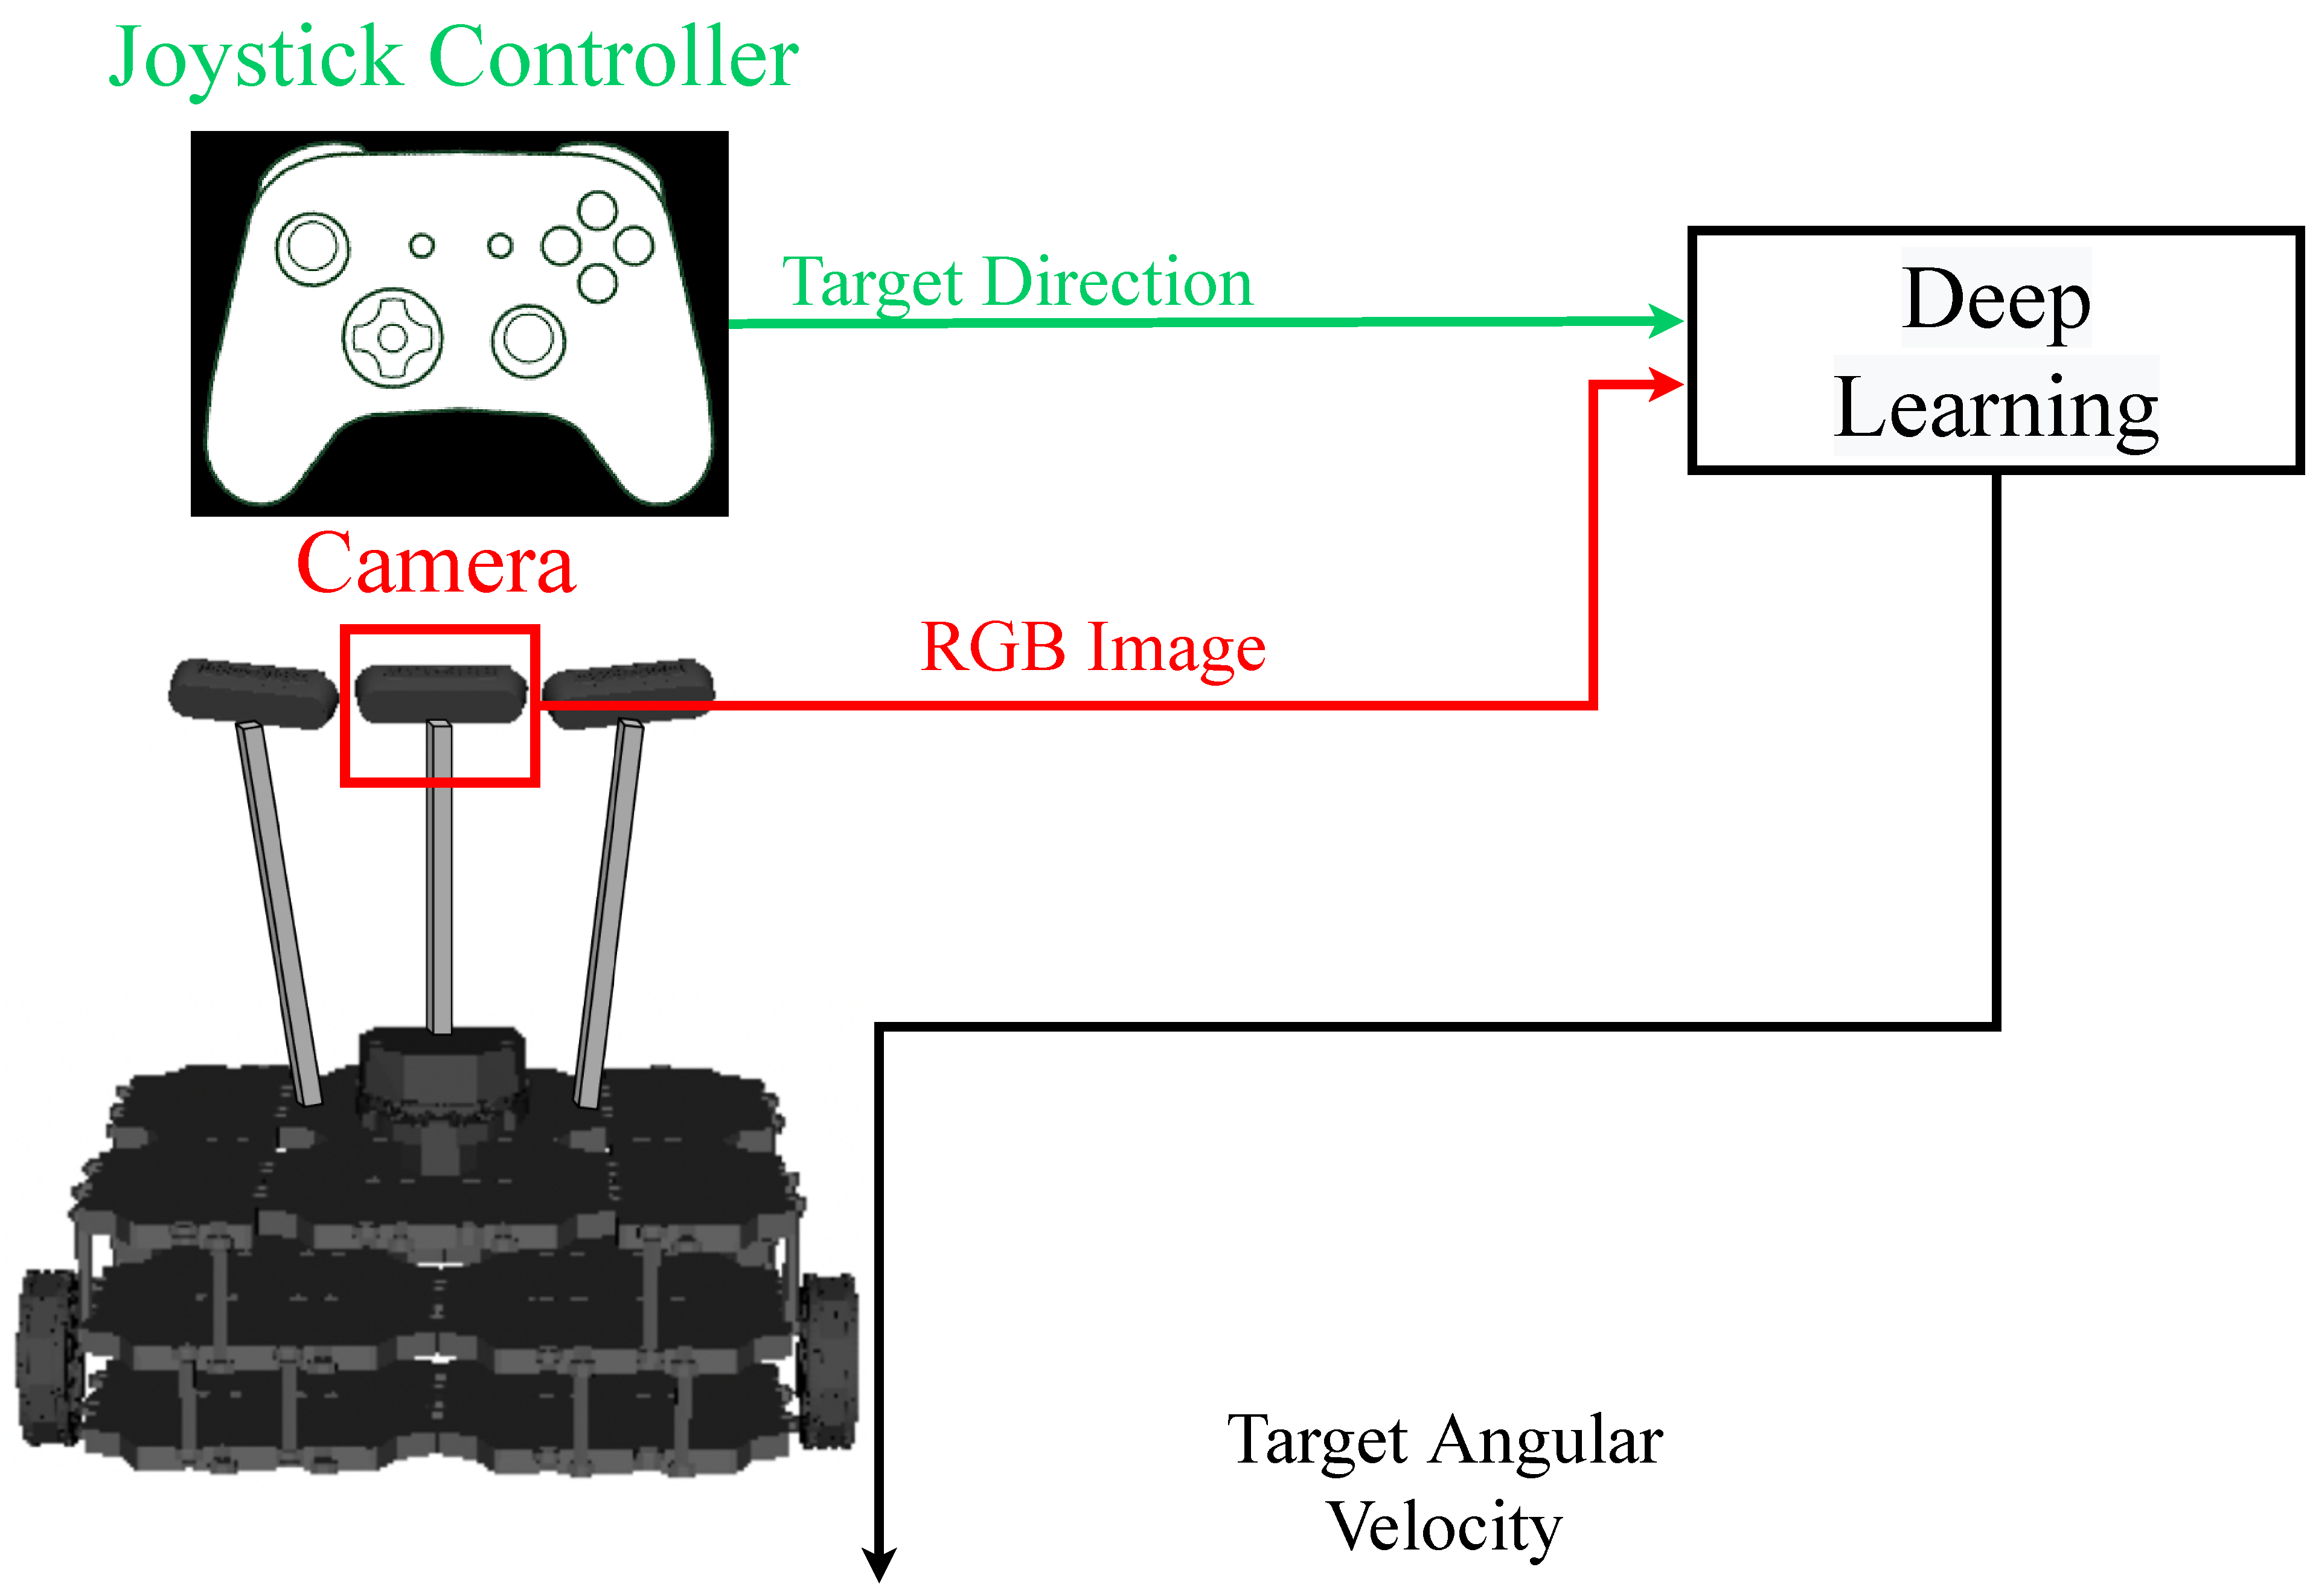
\includegraphics[width = 12cm]{./figs/system_test.pdf}
    \caption{Test system}
    \label{fig::testsystem}
\end{figure}

\newpage
\section{ネットワーク構造}
\label{net}
今回のシステムで用いたネットワークをFig. \ref{fig::methodnetwork}に示す.
また,ハイパーパラメータについてTable \ref{tb::param}に示す.
64×48のRGB画像を入力とする入力層1,畳込み層3,全結合層2層を持つ6層のCNNと,CNNの出力とコマンドを入力する入力層1,
全結合層2.出力層1の全10層の構造になっている.
出力はヨー方向の角速度を連続値である.

\begin{figure}[h]
    \centering
    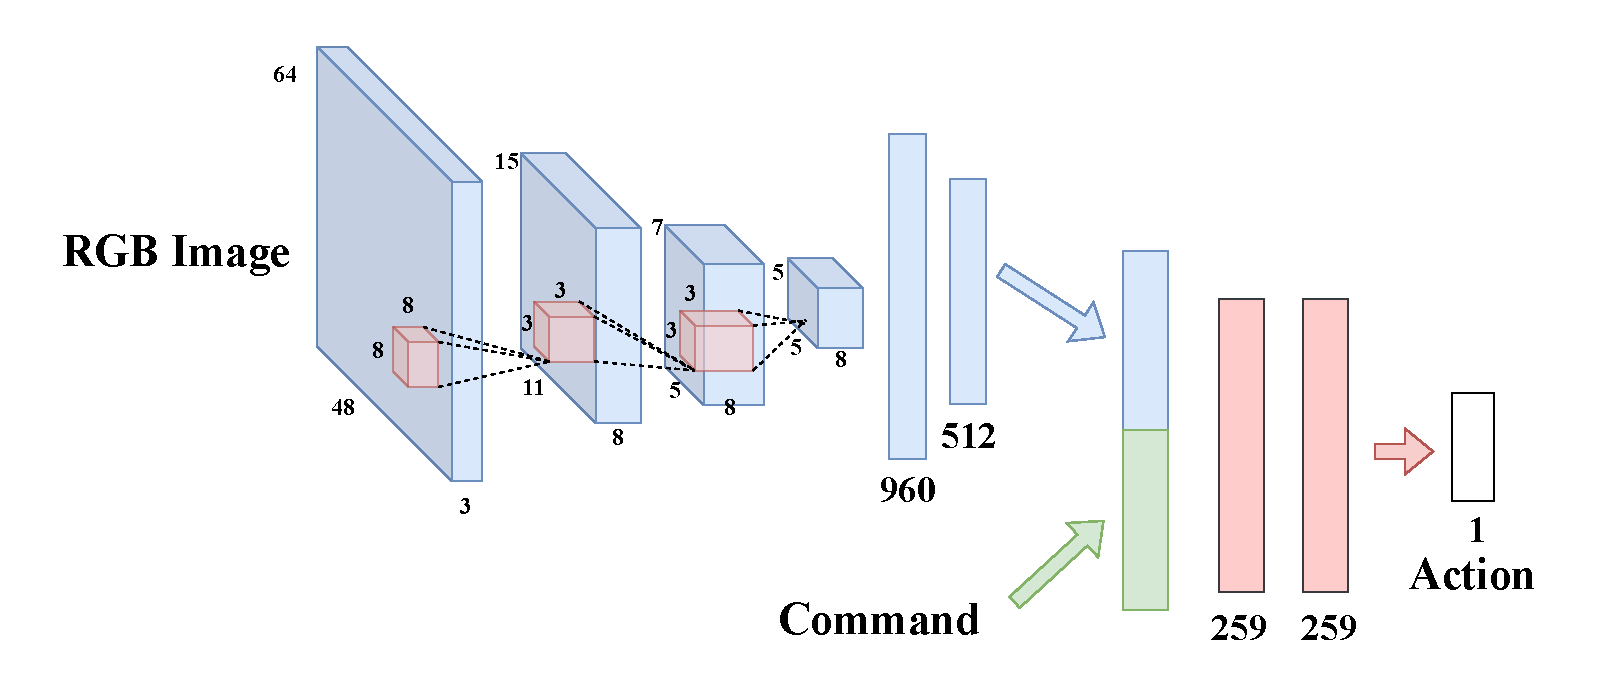
\includegraphics[width = 13cm]{./figs/network.pdf}
    \caption{Method network}
    \label{fig::methodnetwork}
\end{figure}
% \vspace{-1.0zh}
\begin{table}[h]
    \centering
    \caption{Parameters of deep learning}
    \begin{tabular}{|c|c|c|c|}
    \hline
    Input Data    & Image (64x48 pixels, RGB channels) , Command                                              \\ \hline
    Optimizer     & Adam ($alpha = 0.001, beta1 = 0.9, beta2 = 0.999, eps = 1e^{-1}$ )  \\ \hline
    Loss Function & Softmax-cross-entropy                                                            \\ \hline
    Output Data   & Angular velocity                                              \\ \hline
    \end{tabular}
    \label{tb::param}
    \end{table}
\newpage




